\documentclass[a4paper,11pt]{article}
\usepackage[english]{babel}
%\usepackage[cm]{fullpage}			% Fullpage for now
\usepackage[top=2cm]{geometry}
\usepackage[T1]{fontenc}  			% make sure to install cm-super package for improved PDF quality
\usepackage[utf8]{inputenc}
\usepackage{graphicx}
\usepackage[dvipsnames]{xcolor}
\usepackage[font=small]{caption}
\usepackage{subcaption}
\usepackage{microtype}			 	% microtypographical fine-tunning
\usepackage{setspace} 				% Provides support for setting the spacing between lines in a document.
\usepackage{tocbibind}				% Add bibliography/index/contents to Table of Contents.
\usepackage{mathtools}				% enhances amsmath (no need to load amsmath)
\usepackage{amssymb}
\usepackage{amsfonts}
\usepackage{amsthm}
\usepackage{bm} 					% bold math symbols including greek letters
\usepackage{booktabs}				% professional tables (w/o vertical bars)
\usepackage{array}					% 
\usepackage[shortcuts]{extdash} 	% hyphenation of dashed words
\usepackage{cleveref}				% clever environment referencing
\crefname{figure}{Fig.}{Figs.}
\usepackage{siunitx}				% typesetting of SI units
%\usepackage{paralist}		     	% compact lists with more options
% Not sure which to use for bibliography
\usepackage{cite}
%\usepackage{citesort}
%\usepackage[square, sort, numbers, authoryear]{natbib}
\usepackage{pgfplots}
\usepackage{enumitem}
\usepackage{scrextend}

\usepackage{physics}				% Helpfull macros for parens, matrices etc.
\usepackage{xparse}					% Much easier/progressive writing of macros
\usepackage{sty/phdmacros}

% ========================================================

\title{Notes from Self-Driving Car Engineer Nanodegree}
\author{Jakub Prüher}
\begin{document}
	\maketitle
	\section{Motion Models}
	
	\subsection{Constant Turn Rate and Velocity Magnitude (CTRV)}
	Since magnitude of velocity is speed, this model might as well just be called \textbf{Constant Turn Rate and Speed (CTRS)}.

	Differential equation
	\begin{equation}
		\bmqty{
			\dot{p}_x(t) \\
			\dot{p}_y(t) \\
			\dot{v}(t) \\
			\dot{\psi}(t) \\
			\ddot{\psi}(t)
		}
		=
		\bmqty{
			v(t)\cos(\psi(t)) \\
			v(t)\sin(\psi(t)) \\
			0 \\
			\dot{\psi}(t) \\
			0
		}
	\end{equation}
	Using the Euler approximation with \( \Delta t =  t_{k+1} - t_k \)  and the convention \( x_k \triangleq x(t_k) \) we obtain the discretized model described by the difference equation.
	For derivation see Appendix (velocity needs to be assumed constant on interval \( [t_\tind,\ t_{\tind+1}] \) and turn rate is linearized around \( t_\tind \), thus \( \psi(t) \approxeq \psi_\tind + \dot{\psi}_\tind (t - t_\tind) \) ).
	
	\begin{equation}
		\stVar_{\tind+1}
		=
		\stVar_\tind + 
		\bmqty{
			\frac{v_\tind}{\dot{\psi}_\tind}\pqty{\sin\pqty\big{\psi_\tind + \dot{\psi}_\tind \Delta t} - \sin(\psi_\tind)} \\
			\frac{v_\tind}{\dot{\psi}_\tind}\pqty{-\cos\pqty\big{\psi_\tind + \dot{\psi}_\tind \Delta t} + \cos(\psi_\tind)} \\
			0 \\
			\dot{\psi}_\tind \Delta t \\
			0
		}
	\end{equation}
	The state is comprised of 2D Cartesian position \( p_x,\ p_y \), velocity \( v \), yaw \( \psi \) and yaw rate \( \dot{\psi} \).
	\begin{figure}[h!]
		\centering
		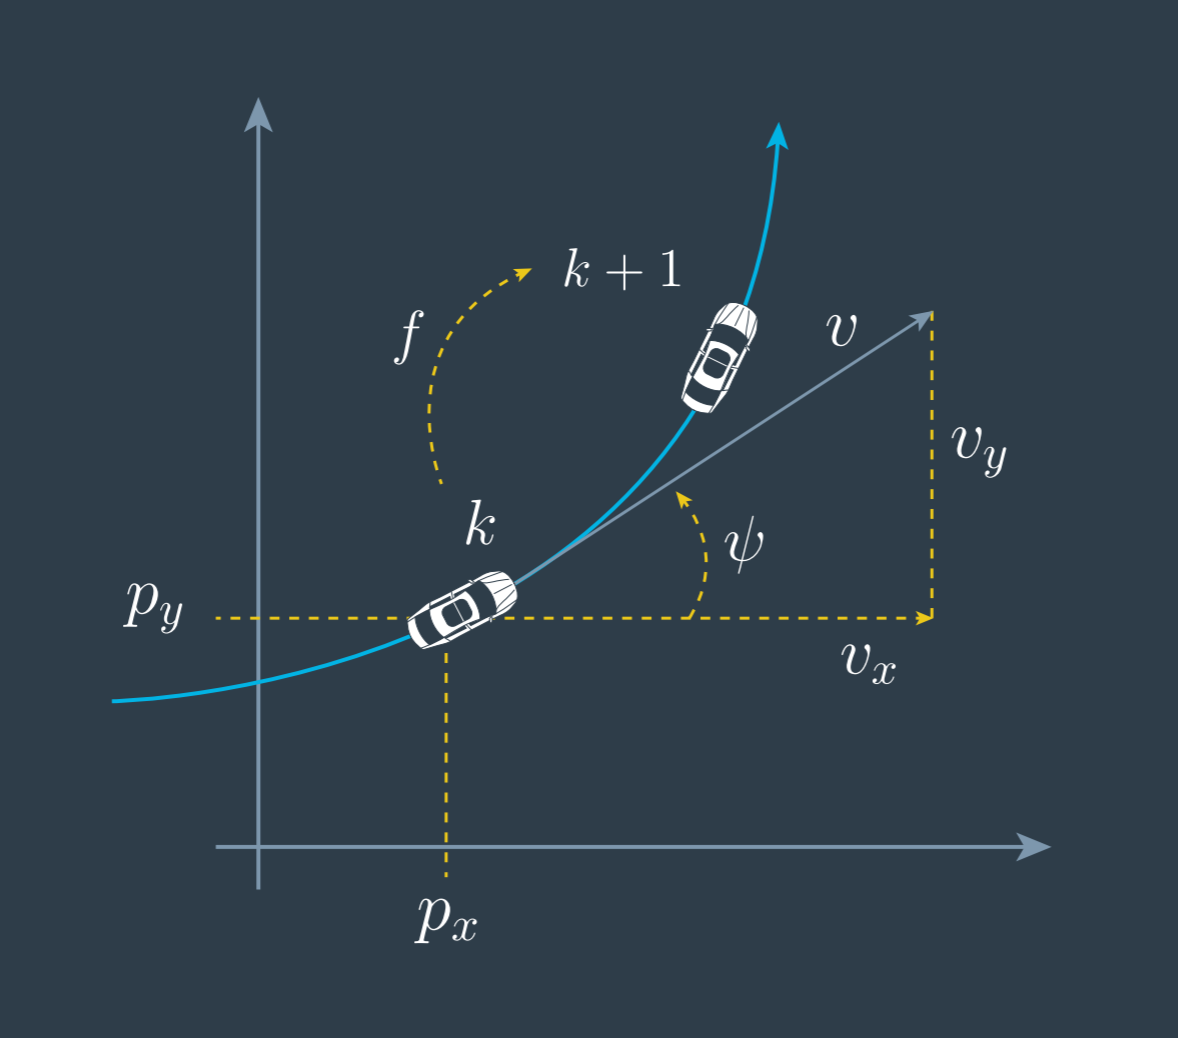
\includegraphics[scale=0.25]{img/ctrv_model}
		\caption{Geometric meaning of the CTRV model variables.}
		\label{fig:ctrv_model}
	\end{figure}
	When the yaw rate is zero, i.e. \( \dot{\psi}_\tind = 0 \), or, yet in other words, the yaw does not change, the model is
	\begin{equation}
		\stVar_{\tind+1}
		=
		\stVar_\tind + 
		\bmqty{
			v_\tind\cos(\psi_\tind)\Delta t \\
			v_\tind\sin(\psi_\tind)\Delta t \\
			0 \\
			0 \\
			0
		}
	\end{equation}
	With the process noise involved the model is
	\begin{equation}
		\stVar_{\tind+1} = 
		\stVar_\tind +
		\bmqty{
			\frac{v_\tind}{\dot{\psi}_\tind}\pqty{\sin\pqty\big{\psi_\tind + \dot{\psi}_\tind \Delta t} - \sin(\psi_\tind)} \\
			\frac{v_\tind}{\dot{\psi}_\tind}\pqty{-\cos\pqty\big{\psi_\tind + \dot{\psi}_\tind \Delta t} + \cos(\psi_\tind)} \\
			0 \\
			\dot{\psi}_\tind \Delta t \\
			0
		} + 
		\bmqty{
			\frac{1}{2}\cos(\psi_\tind) \nu_{a, \tind} (\Delta t)^2 \\
			\frac{1}{2}\sin(\psi_\tind) \nu_{a, \tind} (\Delta t)^2 \\
			\nu_{a, \tind} \Delta t \\
			\frac{1}{2} \nu_{\ddot{\psi}, \tind} (\Delta t)^2 \\
			\nu_{\ddot{\psi}, \tind} \Delta t
		}
	\end{equation}

	Things to note:
	\begin{itemize}
		\item Nonlinear dynamics
		\item The process noise is non-additive
	\end{itemize}

	
	\subsection{How to set process noise covariance?}
	Other models:
	\begin{itemize}
		\item Constant Turn Rate and Acceleration (CTRA)
		\item Constant Steering Angle and Velocity (CSAV)
		\item Constant Curvature and Acceleration (CCA)
	\end{itemize}
	


	
	\section{Sensor Models}
	\subsection{RADAR}
	TODO: range, azimuth and range rate
	
	
	\subsection{LIDAR}
	TODO: Linear model
	
	

	\section{Sensor Fusion}
	Asynchronous measurements: use update with different sensor model each time a  \\
	Synchronous measurements: create a joint model of the RADAR and LIDAR sensors and use it in a regular measurement update
	
% ========================================================
\end{document}

